\section{Runtime Issues and New Methods}

My initial goal was to run my algorithm on real graph datasets.
However, real world datasets of evolving graphs tend to have at least 100,000 vertices.
With my gradient descent algorithm taking $O(n^2 * k)$, where there are $k$ iterations, I was worried about
runtime being an issue.

\begin{figure}
    \begin{center}
        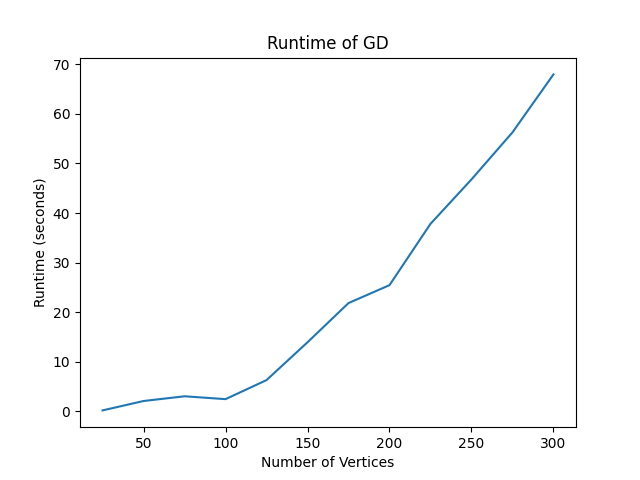
\includegraphics[scale=0.6]{figures/Runtime of Gradient Descent.png}
    \end{center}

    \caption{
        Runtime analysis of Gradient Descent on different sizes of graphs.
    }
    \label{fig:sgd-runtime}
\end{figure}

Following this notion, I decided to perform a test of runtime in Figure ~\ref{fig:sgd-runtime}.
It's clear that this runtime is not likely to be reasonable on anything larger than 1000 vertices.
Therefore, I decided to try other methods to solving the problem.
Continuing in the optimization front, I tried using various methods from scipy's optimization library.
However, this did lead to some issues caused by the ill-posed nature of the problem:

\begin{itemize}
    \item Using automatic differentation would lead to an optimal value of 0 for every spot in $q$.
          This is caused by relaxing $q$ to be a vector instead of a mapping.
          To avoid this, a gradient must be directly provided (leading me to focus on gradient methods like CG and Newton-CG)
    \item To get a result that is very accurate, a gradient algorithm must walk very far down the gradient.
          In particular, my gradient descent walks down the gradient until the magnitude of the gradient is smaller than $10^(-160)$. 
          This leads to many iteration steps (even over 10,000), but this seems necessary to get an extremely accurate model.
\end{itemize}

\begin{figure}
    \begin{minipage}{0.49\textwidth}
        \begin{center}
            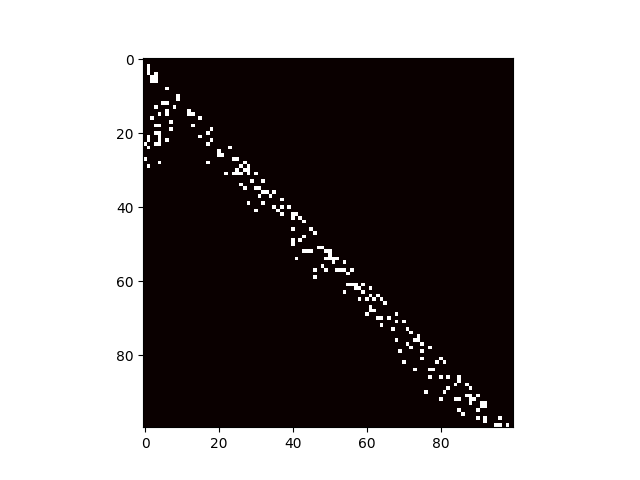
\includegraphics[scale=0.5]{figures/sgd_adj_100.png}
        \end{center}
    \end{minipage}
    \begin{minipage}{0.49\textwidth}
        \begin{center}
            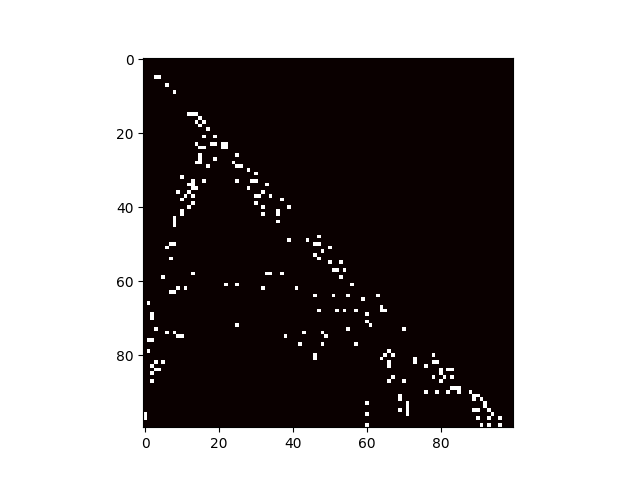
\includegraphics[scale=0.5]{figures/cgnewton-matrix.png}
        \end{center}
    \end{minipage}
	\caption{
        Left: State 200 of the graph with a range mapping learned by gradient descent.
        Right: State 200 of the graph with a range mapping learned by Newton Conjugate Gradient (Newton-CG).
	}
    \label{fig:newton-accuracy}
\end{figure}

\begin{figure}
    \begin{center}
        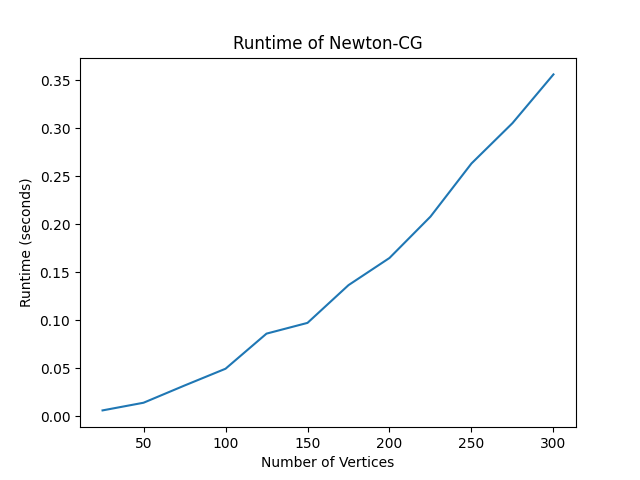
\includegraphics[scale=0.6]{figures/newton-runtime.png}
    \end{center}
    \caption{
        A runtime analysis of the Newton Conjugate Gradient method.
    }
    \label{fig:newton-runtime}
\end{figure}

After testing various optimization methods in the scipy library, I found the Newton Conjugate Gradient method to be the best-performing of them all.
The results of Newton-CG are not nearly as good as my gradient descent results, 
but I think this is because the problem requires walking down such a small gradient for good results.
See Figure \ref{fig:newton-accuracy} for the accuracy of Newton-CG.
The program does converge after less than 100 iterations, and therefore runs far faster than my gradient descent.
So this seems to be a good way to approximate this problem in general for larger datasets.

However, while trying to run larger trials, I actually found that the runtime of generating new states of the graph
and reading in the states of the input took longer than the actual Newton CG method.
This has lead me to the following observations:

\begin{itemize}
    \item A model that is $O(n^2*s)$, where $s$ is the number of states, is far too slow for any social network or internet data.
          This model of birth and death rates per edge cannot hold for such graph sizes.
    \item Most models and algorithms that I know for dealing with normal large graphs deal directly with the sparsity of the graph
          and abuse common structures of the graph (for example, cliques or triangles) 
\end{itemize}

Following these observations, I could not find a dataset that seemed to be a solid fit for this.
The results in~\cite{grindrod2009} apply their method to electroencephalography and they do mention other
very scientific applications, such as protein-protein networks.
However, I am interested in how range-dependent graphs apply to social networks or website data in particular, 
as they don't seem like extremely natural applications.
I am curious to see if these techniques have any chance of applying to such scenarios, even notwithstanding the issue
of problem size.